\chapter{Introduction}\label{chap:intro}
%\begin{epigraphs}
%  %\qitem{\emph{śr̥tiḥ mātā layaḥ pitā} (Tone is the mother, rhythm is the father) says an old adage...}{This dissertation is about daddy issues! Only in draft, to be taken away}
%  %\qitem{Music creates order out of chaos: for rhythm imposes unanimity upon the divergent, melody imposes continuity upon the disjointed, and harmony imposes compatibility upon the incongruous}{Yehudi Menuhin}  
%  \qitem{...the most necessary, most difficult and principal thing in music, that is time...}{W. A. Mozart from \emph{Mozart: The Man and the Artist, as Revealed in his own Words} by Friedrich Kerst, trans. Henry Edward Krehbiel (1906)}
%\end{epigraphs}
%%\note{Chapter in brief: An introduction to thesis, motivating the problem of rhythm analysis with applications, provide a context for the thesis within MIR and within CompMusic, focus on broad approach in the work, mention the main aims and contributions, provide an organization and the best way to read it. Material presented here is derived mainly out of the thesis proposals 2012, 2013, and new learnings in hindsight.}
%%
%%ICT and how they have impacted our lives.
%\noindent We live in a multicultural world that is replete with rich sources of data and information, which keep increasing each passing day. The present day \gls{ICT} and tools help us to generate, organize, interact, interpret, consume, assimilate these data and information, enhancing our experience with the data, information and knowledge of the world. The technology needs in a multicultural world are evolving to cater to the complex sociocultural contexts in which these technologies and tools are being built and used. 
%
%Music is an integral part of our lives and is being produced and consumed at an ever increasing rate. The consumption channels and practices of music have changed significantly over the last two decades. With music going digital, there are large collections of music available on demand to users, necessitating novel ways of automatically structuring these collections. The interaction with music has grown beyond just listening into an enriching and engaging experience with the music content. Such a scenario provides a great opportunity to enhance our experience interacting with music. There are significant efforts to build automatic tools and technologies that enhance our experience with large (and ever increasing in size) music collections. Music being a sociocultural phenomenon needs these automatic tools to be aware and adaptable to such a context and cater to specific music cultures, music producers (musicians and artists) and the widely diverse audiences.
%
%\gls{MIR} is a specialized area of research within music technology that aims to develop tools and applications for representation, understanding, analysis and synthesis of music. Though a new and interdisciplinary field of research, it has a significant community working on various problems within the purview of \gls{MIR}. \gls{MIR} focuses on understanding and modeling what music is and how it functions. Its basic aim is to develop veridical and effective computational models of the whole music understanding chain, from sound and structure perception to the kinds of high-level concepts that humans associate with music, such as melody, rhythm, harmony, structure, mood and other possibly subjective attributes and characteristics. Automatic music analysis in \gls{MIR} aims to `make sense' of music and extract useful, musically relevant and semantically meaningful information from music pieces and music collections. 
%
%Music is multi-dimensional and rhythm is one of the most basic dimensions of music. Music manifests as musical events unfolding in time, and the arrangement of these events constitutes the rhythm of a music piece. These events can be grouped and organized in several layers into rhythmic structures and patterns. Rhythm can be studied from many different perspectives \cite{bello:15:perspective}, and this work takes an \gls{MIR} viewpoint aiming at automatic rhythm analysis: to estimate and characterize these rhythmic structures and patterns from music to extract musically meaningful rhythm related information from music. 
%
%The work presented in this dissertation is at the crossroads of music technology and automatic analysis of music, focusing on rhythm analysis, aiming at domain specific analysis approaches within a multicultural context. We now delve into the context and motivation for the thesis. The scope and objectives of the thesis are then clearly identified. The concluding section of the chapter describes the organization of the dissertation in detail. 
%\section{Context and relevance}
%In the last two decades, \gls{MIR} has received significant attention from the research community and has addressed several relevant research problems advancing the field of sound and music computing. However, the current research in \gls{MIR} has been largely limited to Eurogenetic\index{Eurogenetic music} (popular) music\footnote{The term Eurogenetic music was introduced by \citeA{ajay:14:rhythmJNMR} to avoid the misleading dichotomy of Western and non-Western music. The discussed theoretical constructs of western music are motivated by music of the European common practice period. We use the word ``genetic" rather with its connotation as ``pertaining to origins", coined in 1831 by Carlyle from Gk. genetikos ``genitive", from genesis ``origin", and not in its biological sense as first applied by Darwin in 1859 (\url{http://www.etymonline.com}). The term was proposed by Prof. Robert Reigle (MIAM, Istanbul) in personal communication.} cultures and do not generalize to other music cultures of the world. The approaches have not been developed within a multicultural context and are incapable of extending to the wide variety of music cultures we encounter. 
%
%There is still a wide gap between what can accurately be recognised and extracted from music audio signals and the high level semantically meaningful concepts that human listeners associate with music. Current attempts at narrowing this semantic gap are only producing small incremental progress. One of the main reasons for this lack of major progress seems to be the bottom-up approach currently being used, in which features are extracted from audio signals and higher-level features or labels are then computed by analysing and aggregating these features. The limitation here being the lack of infusion of higher level music knowledge directly into automatic analysis. The CompMusic\index{CompMusic} project \cite{serra:11:compmusic} was conceived in such a context to address these limitations. 
%
%CompMusic \footnote{\url{http://compmusic.upf.edu}} (Computational Models for the Discovery of the World's Music) is focused on the advancement in the field of \gls{MIR} by approaching a number of current research challenges from a culture specific perspective to build domain specific approaches. CompMusic aims to  develop information modelling techniques of relevance to several non-Western music cultures and in the process contributing to the overall field of \gls{MIR}. Five different music cultures are being studied in the project: Hindustani (North India), Carnatic (South India), Turkish-makam (Turkey), Arab-Andalusian (Maghreb), and Beijing opera (China). 
%
%CompMusic aims to challenge the current Western centered information paradigms, advance our information technology research, and contribute to our rich multicultural society. The motivation behind CompMusic is that the information technologies used for music processing have typically targeted the western music traditions, and current research is emphasizing this bias even more. However, to develop technologies that can deal with the richness of our world's music, there is a need to study and exploit the unique aspects of other musical cultures. 
%
%CompMusic further identifies that `making sense' of music is much more than decoding and parsing an incoming stream of sound waves into higher-level musical objects such as onsets, notes, beats, melodies and harmonies. Music is embedded in a rich web of cultural, historical, commercial and social contexts that influence how it is interpreted and categorized. Though all music traditions share common characteristics, each one can be recognized by particular features that need to be identified and preserved. Many qualities attributed to a piece of music by listeners and musicians cannot solely be explained by the content of the audio signal itself. It is clear that high-quality automatic music description and understanding can only be achieved by also taking into account additional information external to the music. %This also constitutes a fruitful opportunity for interdisciplinary research involving engineers, musicians, musicologists and psychologists to collaborate and contribute their valuable knowledge.
%
%Looking at the problems emerging from various musical cultures will not only help those specific cultures, but we will open up our existing computational methodologies, making them much more versatile. It will emphasize the limitations of the current methodologies and present open issues. In turn, it will also help preserve the diversity of our world's culture. The research results of CompMusic are integrated into Dunya~\cite{porter:13:dunya}, which is a web-based software application that lets users interact with an audio music collection through the use of musical concepts that are derived from a specific music culture. The users can also access all the research results and extracted features through Dunya. % through a web API. 
%
%Within the field of \gls{MIR} there are many research problems that can benefit from a culture specific perspective. CompMusic focuses on the extraction of features from audio music recordings related to melody and rhythm, and on the semantic analysis of the contextual information of those recordings. The goal is to characterize culture specific musical facets of each repertoire and to develop musically meaningful similarity measures with them. The research in CompMusic is data-driven, thus it revolves around corpora. One of the goals of CompMusic is to construct a research corpus for each music tradition~\cite{serra:14:corpus}. The types of data gathered are mainly audio recordings and editorial metadata, which are then complemented with descriptive information such as editorial metadata, scores and/or lyrics as available. 
%
%The work presented in this dissertation has been conducted in the context of the CompMusic project but focusing on automatic rhythm analysis research problems for Indian art music from a data-driven perspective using signal processing and machine learning approaches. The dissertation imbibes and inherits all the goals and context of CompMusic project as applied to rhythm analysis. A meaningful automatic rhythm analysis hence should consider cultural aspects attached to it~\cite{serra:13:roadmap}. Through a culture-aware and domain specific approach to computational rhythm modeling of Indian art music, we will also get better insights into the current \gls{MIR} tools which would improve their performance. We will be able to develop better algorithms, newer methodologies and techniques for the study of world's music and reach out to a much larger part of our multicultural world. The development of these models would also allow cross cultural comparative studies between different musical systems, enriching the present knowledge of world's music and provide interesting sociocultural, cognitive, and musical perspectives. Such an approach is relevant since it aims to push ahead the boundaries of automatic rhythm analysis to address current challenges and be more inclusive to address varied needs of different music cultures of the world. 
%\section{Motivation}
%Rhythm is a fundamental dimension of music. Music has repeating structures and patterns, with several musical events organized in time. It is primarily an event-based phenomenon and detecting and characterizing musical events and their transitions is an important task. The automatic analysis of these musical events can provide us useful insights into music and help us to derive semantically meaningful higher level concepts. 
%
%Musical events are often organized in several hierarchical layers leading to metrical structures\index{Meter}. The metrical structures provide a fundamental framework in time to organize events and hence play a pivotal role in music. Most melodic and rhythmic phrases, lyrical lines, and harmonic changes are organized around metrical structures and hence the estimation of different aspects of the meter is an important \gls{MIR} task. Estimating the note onsets, tempo, beats and downbeats are useful and necessary for any further analysis of music. Though each of these aspects can be extracted in an isolated fashion, there is significant interplay between these entities and hence a holistic approach to describing all these aspects of meter is an approach that needs to be explored further. 
%
%There are additional structures often in music at a longer time scale than the metrical structures. These are structural components (e.g. verse, chorus, bridge, intro, outro, solo) and are well defined in many music forms as different sections of a music piece. Segmenting a song at these section boundaries is also a useful task for summarizing the audio or for structural analysis of music pieces. Such a structural analysis can benefit from metrical analysis of a music piece since most of these sections are aligned with metrical boundaries in a song. 
%
%Music is also replete with rhythmic patterns at several different levels. Music is expressed through a grouping of events into rhythmic patterns\index{Rhythm pattern} and hence these patterns are fundamental to understanding rhythm. The rhythmic patterns can also be indicative of the underlying musical structure. Understanding and analysis of these patterns would help in a comprehensive computational description of the music piece and can be further used in several applications. 
%
%Analysis of rhythmic structures and patterns hence is an important research task in \gls{MIR}. Tools developed for rhythm analysis can be useful in a multitude of applications such as intelligent music archival, enhanced navigation of music collections, content based music retrieval and for an enriched and informed listening of music. The target audience for such tools span across serious music listeners who wish for an enhanced experience with music, music students who wish to learn more about the music they are listening to, musicians who can use these tools to better promote their music, musicologists who can use these tools in their work, and music collectors and record labels who can use these tools to organize, archive and present their music better. % All these tools will further be integrated into Dunya, a culture aware music navigation 
%
%With large and ever growing music collections, the need of the hour are innovative ways for meaningful organization and navigation through these large collections. Large music collections would mean an automatic analysis is desired over a manual curation that can be tedious, time consuming and highly resource intensive. In addition to the metadata associated with music recordings, using the underlying musical concepts to organize music collections is the best approach in such a case for better search and discovery within the collection. This necessitates defining similarity (or distance) measures between these recordings that can be used to group and collate recordings. In addition to the context based similarity (that uses mainly editorial metadata) that is predominantly used today, there is a need to develop content based similarity (using music content of the audio recordings). Further, navigating within a recording would also mean that these similarity measures are additionally needed intra-piece i.e. for different parts of a single piece. 
%
%As specified earlier, a meaningful navigation and retrieval can be better achieved using the sociocultural context of the music with all its unique features and specificities - using culture specific similarity measures. Rhythmic features are a component of the overall similarity measures for such a task and rhythm similarity\index{Rhythm similarity} measures can hugely benefit from automatic rhythm analysis of rhythmic structures and patterns. The culture specificity applies at several levels - it applies to identifying unique challenges for the current day \glspl{ICT} making them specific and meaningful, applies to research approaches for automatic analysis of music, and to the methodologies of combining information from several data sources to define meaningful similarity measures. 
%
%With a significantly sophisticated rhythmic framework, Indian art music poses a big challenge to the current state of the art in automatic rhythm analysis \cite{ajay:14:rhythmJNMR}. There are several important automatic rhythm analysis tasks in Indian art music that have not been studied. With such complexities, developing approaches for rhythm analysis in Indian art music can help to identify the limitations of current approaches to improve their performance and make them better and more general. As emphasized earlier, there is a significant gap between the current capabilities of the music technologies used in commercial services and the needs of our culturally diverse world. This is evident in Indian art music - where the existing technologies fall short of utilizing even the basic musical characteristics and limit our music listening experience. Being well established art music traditions with a significant audience around the world, Indian art music traditions are ideal candidates to develop culture-aware automatic rhythm analysis methods. 
%
%It is important to comment that in the pursuit of culture specific methodologies, it is illusionary to believe that specialist systems can be developed for each of the musics of the world. Therefore, a more rational approach is to develop culture-aware methods that are also generalizable and adaptable to other contexts and musics. 
%
%The motivation for culture-aware automatic rhythm analysis in Indian art music stems from all the above described reasons. In addition to the above, to the best of our knowledge, this is the first thesis to comprehensively address automatic rhythm analysis problems in Indian art music and hence would open up the way for further research on the topic. Being an unexplored area of research with many different open problems, it is important and necessary to clearly identify the scope and objectives of this dissertation. 
%\section{Scope and objectives}
%The work presented in the dissertation on automatic rhythm analysis stands at the intersection of audio music processing, machine learning, music theory, musicology, and the application of enriched music listening. Automatic rhythm analysis is itself a broad area of research and hence it is quite necessary to define and delimit the scope of the research presented in the dissertation, while identifying the research questions and the objectives of the thesis clearly. The broad objectives of the presented research are listed below:
%\begin{itemize}[leftmargin=*]
%\item To identify challenges and opportunities in automatic rhythm analysis of Indian art music and formulate relevant automatic rhythm analysis problems. Convert musical definitions into engineering formulations amenable to quantitative analysis using signal processing and machine learning approaches. 
%\item To build useful annotated music collections of Indian art music (both audio and symbolic) with a focus on rhythm, for future research in automatic rhythm analysis
%\item To create and construct culture-aware computational rhythm models for Hindustani and Carnatic music
%\item To develop novel signal processing and machine learning methods for rhythm analysis of Indian art music
%\item To devise and develop musically meaningful rhythm similarity measures for a better structuring and discovery of Indian art music music collections
%\item To explore extensions and generalizations the specific models to other relevant music cultures being studied in the context of CompMusic project, such as Beijing opera and Turkish makam music. 
%% \item To develop applications and tools for enhancing people's experience with rhythm in specific. 
%\end{itemize}
%
%\noindent To explain the scope of the thesis, a long and comprehensive title that defines the scope of the work presented can be written as: 
%\begin{quote} 
%  \noindent \textit{Culture-aware and data-driven signal processing and machine learning approaches for automatic analysis, description and discovery of rhythmic structures and patterns in audio music collections of Indian art music}
%\end{quote}
%In alignment with the goals of CompMusic, the final goal of such an analysis is to define culture specific and musically meaningful rhythm similarity measures within a music repertoire. The main focus of the thesis is on Indian art music. While there are three other music traditions under study in CompMusic project, the thesis only aims to explore extensions to some relevant rhythm analysis problems in Beijing opera. 
%
%The thesis explores data-driven engineering approaches for analysis of audio music recordings. An audio recording is hence the primary source of information and is at the centre of analysis, with several types of rhythm related information extracted from a recording. \figref{fig:intro:rhythmanalysis} shows an example of such a paradigm, showing meter, patterns and structure extracted from an audio recording of a music piece. Other possible media of music dissemination such as scores, lyrics and contextual information are considered secondary sources in the scope of the thesis, though used in some tasks. The approaches taken in the thesis are primarily audio signal processing and Bayesian machine learning methods, exploring mostly supervised learning methods to develop novel rhythm analysis algorithms. Semantic analysis, which is the other core research area of CompMusic is not the focus of this thesis.
%\begin{figure}
%\centering
%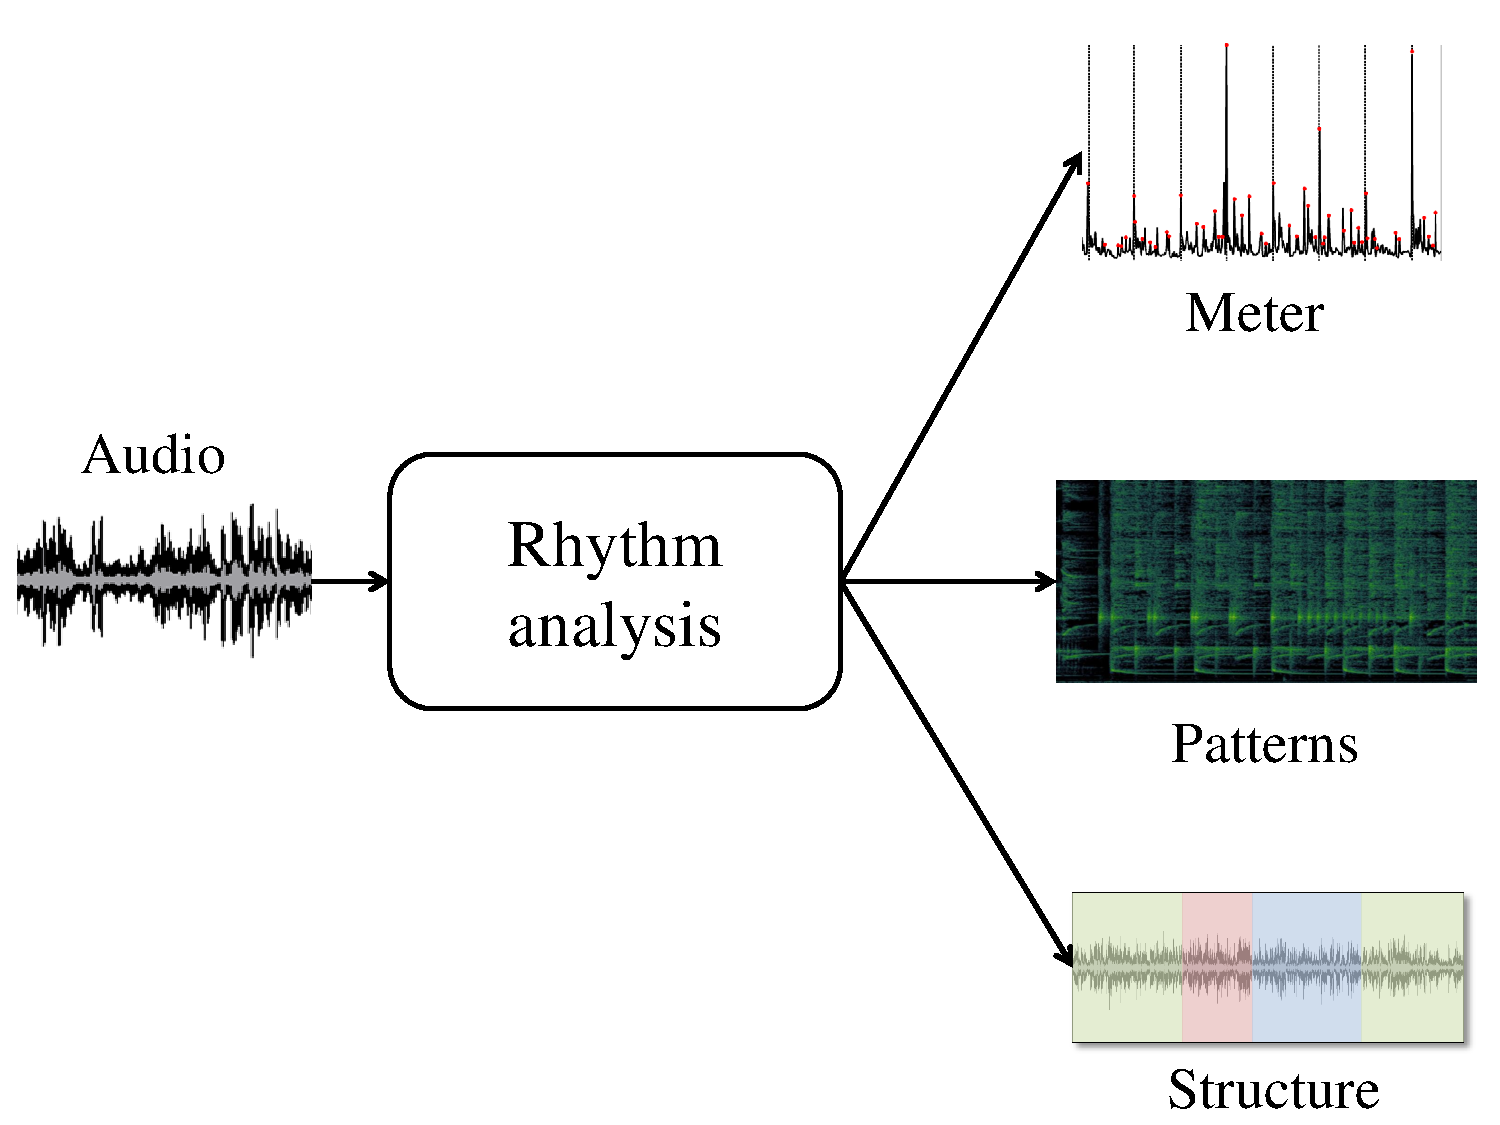
\includegraphics[width=0.9\textwidth]{figs/blockDiags/rhythmAnalysis.pdf}
%\caption[Automatic rhythm analysis from audio]{Example of automatic rhythm analysis from audio recordings estimating meter, rhythmic patterns and structure from audio recordings. The approaches in the dissertation follow a similar flow, with an audio recording being at the centre of analysis.}\label{fig:intro:rhythmanalysis}
%\end{figure}
%
%The thesis aims to bring in as much musical knowledge to the methods as possible, including and using all the known attributes of music. The goal is to build domain specific and informed signal processing and machine learning methods, so that the extracted information is musically relevant and useful. Bayesian models\index{Bayesian model} and methods provide an effective framework to bring in higher level music knowledge into models, in terms of model structure and priors. Bayesian models are hence a central theme for the analysis approaches in the thesis. 
%
%The emphasis of the thesis is on data and methods. The data-driven approaches need good quality datasets, which have been careful compiled and annotated within the context of the thesis. The algorithms are built to work on real world representative music collections - organized curated collections of music that are accessible. 
%
%The thesis focuses only on music analysis and not on music generation, composition and synthesis. The generative models used for analysis in the thesis can however be used for such a task if needed, though it is not the focus of the thesis. In terms of our interaction and experience with music, the thesis focuses mainly on enhanced music listening. Though some of the tools and methods can be useful to both teachers and students of music, it is not the focus of the thesis. 
%
%The work presented is done on well studied art music cultures of India and borrows from the significant musicological literature already available. The thesis however aims to aid musicologists further in their work with these rhythm analysis tools. The data and the methods presented in the thesis can be used by musicologists for large scale corpus level musicological analysis. There are illustrative examples of such analyses in the dissertation, but the thesis does not aim to make any significant musicological conclusions. 
%
%The work in the thesis also borrows from consultation with several musician collaborators over the course of CompMusic project. The analysis methods developed in the thesis do not aim to replace expert musician opinions, but only work within the framework provided by musicians, musicologists, listeners and learners to enhance our experience with music. The problems formulated and addressed in the thesis are on concepts that have well grounded definitions and agreement among the musician and musicologist community. 
%
%In addition to exploring novel approaches to automatic rhythm analysis, the thesis aims to answer the following research questions within the context of rhythm analysis: 
%\begin{enumerate}[leftmargin=*]
% \item It is hypothesized that automatic analysis of rhythmic structures and patterns from audio signals needs specific methodologies that make use of the knowledge about the underlying rhythmic structures. To what extent does incorporating higher level knowledge affect the performance of automatic analysis algorithms? What kinds of higher level information are useful and lead to a better performance? How can such higher level information be included in the framework of Bayesian models to develop novel rhythm analysis algorithms? 
% \item How do the existing rhythm analysis methods designed with different rhythmic structures extend to complex metrical structures in Indian art music? What limitations can we identify of the existing state of the art? 
% \item It is hypothesized that instead of a component-wise disjoint approach to estimating different components of rhythm, it might be useful to jointly estimate all the relevant components together in a single framework. The methods can then utilize the interplay between the components for better estimation. Does a holistic approach work better or is it better to estimate individual components separately? Which components of rhythm are better estimated jointly, and which components can be independently estimated?
% \item It still remains an open question if we need more specialist approaches, or more general approaches that are able to react to a large variety of music. Generally, it appears desirable to have generic approaches that can be adapted to a target music using machine learning methods. What are some such methods, and how can they be useful to adapt it to different music cultures? 
% \item Indian art music and several other music traditions of the world have developed syllabic percussion\index{Syllabic percussion} systems for transmission of their repertoire and technique, which provide a language for percussion in those music cultures. What is the utility of these syllabic percussion systems in automatic percussion pattern analysis? 
% \item Given the availability of useful annotated datasets, one of the questions to ask is if the annotations and the data can be used for a corpus level analysis leading to meaningful and valid musicological conclusions. 
%\end{enumerate}
%
%Broadly, the thesis identifies the challenges and opportunities in automatic rhythm analysis of Indian art music, formulates several rhythm analysis tasks, addresses the issues with building datasets for rhythm analysis, and then focuses on the tasks of meter and percussion pattern analysis. 
%
%The scope of the thesis within CompMusic is to provide rhythm analysis tools and methods to be a part of the comprehensive set of content based analysis methods for the music cultures under study, with the final goal of utilizing these analysis methods to define musically relevant similarity measures. 
%
%A major strategy of CompMusic is open and reproducible research - to be open in sharing ideas, goals, results, data and code as widely as possible. All the data, code and results presented in the thesis will be available openly or be accessible to the research community. Whenever possible, resources will be provided to reproduce the results of the thesis. The data and code will be shared with the community through open source platforms under open licenses. An open dissemination strategy is one of the primary objectives of the thesis. 
%% \comment{Write about the broad tasks addressed in the thesis, so that Chapter 2 (background) has a better context.}
%\section{Organization and thesis outline}
%The dissertation has seven chapters. Each chapter is written on a major topic of the thesis and is aimed to be self contained with a short introduction, content, and a summary. The writing style followed in the thesis is a mixture of both active and passive voice. Most of the dissertation derives content from published research papers describing the work done by collaborative teams. Hence the word `we' refers to the author and when applicable, additionally includes the co-authors and collaborators in research papers. When presenting results and making observations, the word `we' further includes the reader who can equally make such an observation from the results. However, the main original contributions by the author of the thesis are emphasized appropriately, wherever needed. 
%
%After an introduction to the thesis in \chapref{chap:intro}, \chapref{chap:bkgnd} provides an overview of the music background and a review of the state of the art as needed for the thesis. \chapref{chap:probdef} is focused on identifying and discussing several novel automatic rhythm analysis problems in Indian art music. \chapref{chap:datasets} presents the research corpora and all the rhythm related datasets compiled as a part of CompMusic project that will be used for various rhythm analysis tasks. \chapref{chap:meterInfTrack} and \chapref{chap:percpatt} are the main chapters of the dissertation discussing the topics of meter analysis and percussion pattern discovery, respectively. \chapref{chap:conclusions} presents some of the applications and conclusions with pointers for future work. In addition, the links to resources from the thesis (data, code, examples) are listed in \appref{app:resources}. There are several new non-standard terms in the dissertation including unfamiliar terms related to Indian art music which are all listed with a short description in a glossary in \appref{app:glossary}. The glossary also lists the acronyms used for datasets and analysis methods in the dissertation. 
%
%\chapref{chap:bkgnd} provides an overview of the background material necessary for the thesis. It introduces a concrete terminology for rhythm concepts and a basic introduction to rhythm and percussion in Indian art music and Beijing opera. It then provides an overview of the state of the art for automatic rhythm analysis in \gls{MIR}. The chapter ends with a brief overview of the technical concepts useful to understand the thesis work better. The content of the chapter is compiled and presented from several external sources cited appropriately when necessary. 
%
%\chapref{chap:probdef} identifies several challenges and opportunities to automatic rhythm analysis in Indian art music. The chapter aims to present all identified relevant research problems, while only a subset of them are addressed in the thesis. For these problems, the chapter also presents an overview of the state of the art when available. It further elaborates and formulates the thesis problems that are addressed in detail in the next chapters of the dissertation and presents an evaluation of the state of the art for some of these tasks on Indian art music. A large part of the content of the chapter is derived from several discussions of with collaborators of CompMusic, musicians, musicologists and listeners on what they consider are important rhythm analysis problems, with some content and results from our published journal article \cite{ajay:14:rhythmJNMR}. 
%
%\chapref{chap:datasets} describes the efforts of CompMusic in compiling and annotating the research corpora and test datasets. The chapter presents a systematic framework to elucidate a set of design principles to build data corpora for research in Indian art music \cite{serra:14:corpus}. All the annotated rhythm related datasets are described in detail emphasizing on the research problems in which they are useful. Other state of the art datasets that are used in the thesis are also described. Apart from being useful as test datasets to evaluate algorithms and approaches, annotated datasets are also useful to infer musically meaningful observations. Hence an illustrative corpus level statistical analysis of relevant test datasets is also presented to point out some interesting observations. The rhythm related datasets described in the chapter have a major contribution from the author, but still are collective efforts of the CompMusic team, as indicated with each dataset. Some of the content of the chapter is from our published papers~\cite{ajay:14:smc,ajay:14:talaTrack,tian:14:icassp,ajay:14:ismirbo,gupta:15:tabla,ajay:16:spmodel} while some of it is unpublished content. 
%\begin{figure}
%\centering
%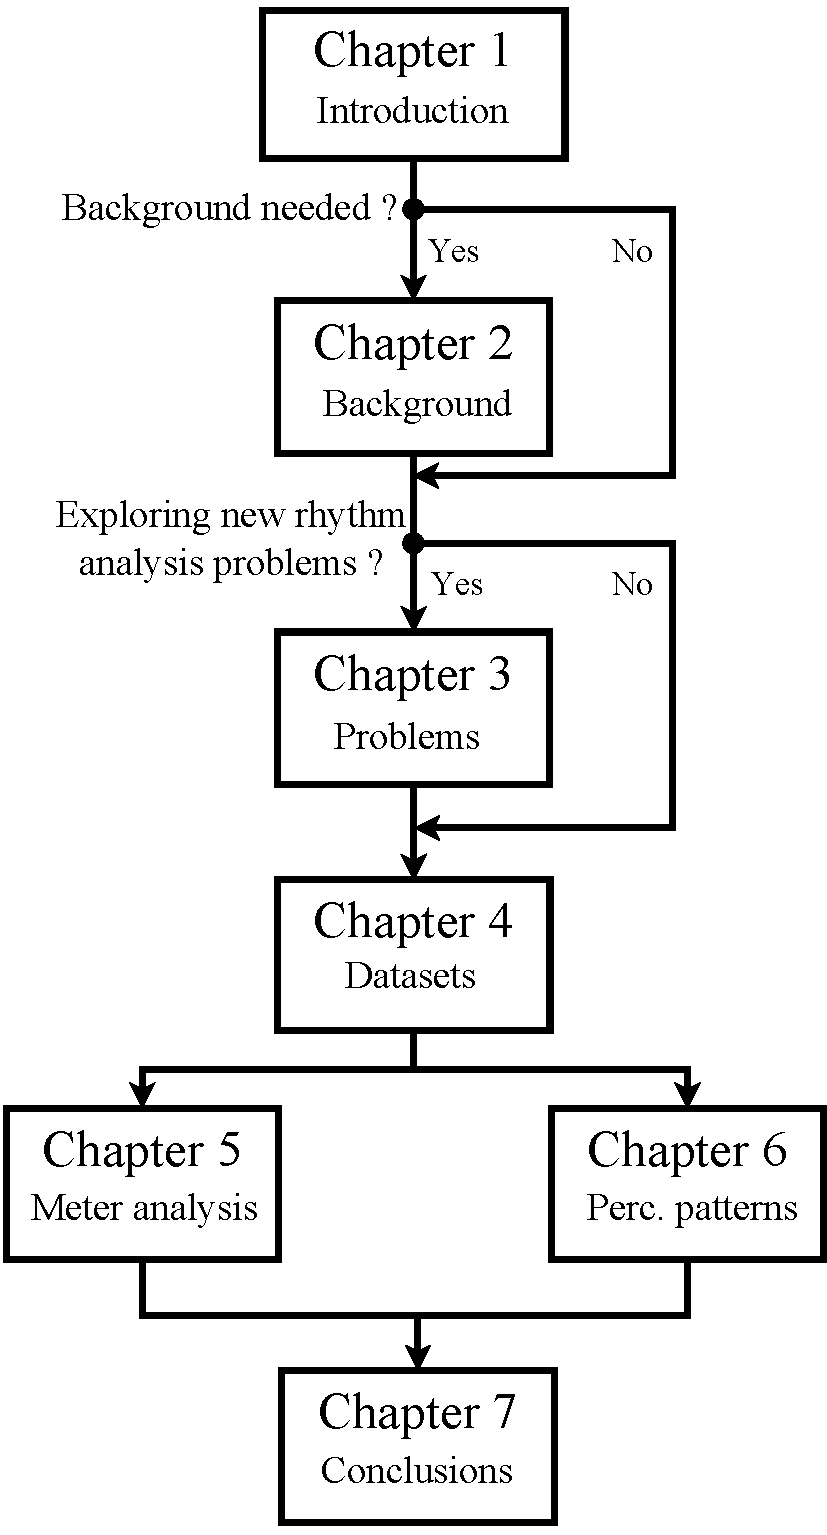
\includegraphics[scale=0.52]{figs/blockDiags/chapterOrg.pdf}
%\caption[Dependencies between the chapters of the dissertation]{Dependencies between the chapters of the dissertation, also indicating a suggested reading order for the chapters}\label{fig:intro:chapread}
%\end{figure}
%
%\chapref{chap:meterInfTrack} presents the primary contribution of the thesis and describes one of the main research problems addressed. The chapter focuses on the problem of meter analysis and describes several approaches to the task in the context of both Carnatic and Hindustani music of India. The chapter proposes novel Bayesian models and novel inference algorithms for different levels of informed meter analysis, with a comprehensive evaluation on annotated datasets. The content of the chapter is derived from the current state of the art in beat and downbeat tracking~\cite{krebs:13:bpm,krebs:15:pf}, along with some of our recently published papers~\cite{ajay:14:talaTrack,ajay:15:pf,ajay:16:spmodel,holzapfel:14:odd} and from latest unpublished work. 
%
%\chapref{chap:percpatt} presents the other important contribution of the thesis and describes the task of percussion pattern discovery in Indian art music. The work presented in the chapter is preliminary and exploratory, but demonstrates the effective use of syllabic percussion systems in representation, transcription and search of percussion patterns in percussion solo recordings. As a preliminary test case, experiments on percussion pattern classification in Beijing opera are presented. The approaches are extended to Indian art music and an evaluation is provided on drum solo datasets. A part of the results presented in the chapter are derived from our published papers \cite{gupta:15:tabla,ajay:14:ismirbo} while many results are yet unpublished. \chapref{chap:conclusions} presents some of the applications and conclusions. The chapter summarizes the results from different chapters and presents pointers for future work. 
%
%Each chapter of the dissertation is self contained and can be read in isolation with sufficient background. However, the following dependencies exist between chapters, which is a possible indicator of the recommended order for reading and is further summarized in \figref{fig:intro:chapread}. Starting with \chapref{chap:intro}, if the reader has sufficient background on rhythm in Indian music and rhythm analysis problems in \gls{MIR}, \chapref{chap:bkgnd} would be a recap. For a researcher starting out and exploring new problems and resources in Indian art music, \chapref{chap:probdef} and \chapref{chap:datasets} might be more interesting. \chapref{chap:meterInfTrack} and \chapref{chap:percpatt} focus on separate research problems and can be read independently. \chapref{chap:datasets} might be necessary to understand the evaluations presented in \chapref{chap:meterInfTrack} and \chapref{chap:percpatt}. \chapref{chap:conclusions} might be useful to understand some of the applications in more detail. \appref{app:resources} and \appref{app:glossary} can be used as quick guides for resources and term definitions, respectively. 
%
%To the best of our knowledge, this dissertation is the first comprehensive attempt at rhythm analysis of Indian art music. By addressing the problems discussed in this dissertation within the context of CompMusic project, we aim to develop useful tools and algorithms for automatic rhythm analysis of Indian art music. Integrated into Dunya, we hope that these tools will provide an enriched experience to a music listener, enhanced through a cultural context. In the process, we also hope to obtain a better understanding and provide deeper insights into the nature of rhythm in Indian art music, and contribute to improving the state of the art in \gls{MIR}. 

\noindent We live in a world with explodingly increasing data and information. The \gls{ICT} help us assimilate, organize, interpret, interact, consume and generate these data and information, enhancing the experience with knowledge of the world. The technologies keep developing to follow the fast-evolving sociocultural context, in which we build tools and devise new methods.

Music is a necessary part of many people's lives. Teaching and learning music is not only a hobby but a professional commitment of many people. The knowledge-learning experience has been updating rapidly in the past few years along with the fast developing \gls{ICT}s. A large amount of amateur or professional learners are converted into the online education environment, thus benefited from its easy-accessibility, various course content, and most importantly, the automatic practice assessment feedback which is used to keep the learners aware their shortcomings and gets their skill improved. Music performance, as a type of knowledge and skill, although different and more abstract than other subjects. Its online learning requires automatic tools to adapt to such context and widely diverse learners.

Music Information Retrieval (MIR) is a specialized field within the music technology, in which people invent and develop methods and tools to analyze, synthesize, understand and represent the music. It aims to explain the music concepts at various levels and build computational models for the human music perception and understanding aspects, such as melody, rhythm, timbre, harmony, structure, mood. Automatic music performance assessment in \gls{MIR} aims to extract perceptual and semantic representations in music performance recordings and devise computational models for the performance assessment.

Music has many elements. The singing voice is one of those elements which plays the central role in songs, and it's the main attraction for listeners. The pronunciation aspect of the singing voice is essential in many music traditions as it conveys the semantic information of the lyrics and the aesthetic pleasure to the listeners. This work takes the \gls{MIR} point of view dealing with automatic singing voice assessment and focusing on the pronunciation aspect: to segment pronunciation meaningful singing voice events, extract pronunciation meaningful representations and develop computational models to detect the mispronunciation and measure the pronunciation similarity.

The work presented in this dissertation lies in the automatic music performance assessment subject of the \gls{MIR} field, aiming at domain-specific analysis and assessment approach within a culture-specific context. We now reach the context and motivation of the thesis. The scope and objectives are then defined. Finally, we describe the organization and thesis outline. 

\section{Context and relevance}

In the last two decades, many new methods, models and algorithms have been developed in the \gls{MIR} community, which significantly promoted the advancement of the fields of sound and music computing, and music technology. Initially, the \gls{MIR} research has been restrained to eurogeneric music. Not until recently, we witness an increasing amount of researchers who devote themselves to the \gls{MIR} research of non-eurogeneric music. The CompMusic project plays an essential role in boosting this trend.

CompMusic (Computational Models for the Discovery of the World's Music) is focused on the advancement in the field of \gls{MIR} by approaching new challenges from a culture-specific perspective. CompMusic aims to develop computational models for several non-western music traditions and in the meantime, advance the overall development of \gls{MIR}. CompMusic studies five music traditions: Jingju (also known as Beijing opera, China), Hindustani (North India), Carnatic (South India), Turkish-makam (Turkey), and Arab-Andalusian (Maghreb).  The current information technologies in \gls{MIR} field are typically targeting to solve the problems emerging from the western music. However, a wide range of music traditions other than western music can bring many new challenges. The motivation behind CompMusic is to face these new challenges by studying the five non-western music traditions, and to develop \gls{MIR} technologies to embrace the richness of the world's music.

CompMusic further aims to understand music both perceptually and semantically. The typically \gls{MIR} methods revolve around the audio-centric idea, which parses the incoming audio into high-level music events or concepts, such as onsets, notes, beats, melodies and chords. Although all music traditions share some common concepts, each one has its unique perceptual or semantic attributes that require different interpretations. Additionally, music is encapsulated in a complex sociocultural and historical context, which affects deeply the way of how we interpret it. Many attributes of the five non-western music traditions studied in CompMusic project cannot be explained by the audio or the western music knowledge themselves. Thus, a deeper understanding can only be achieved by considering additional culture-specific information.

Delving into the problems brought by diverse music traditions will not only help develop technologies for the specific tradition, but also will extend the scope of the existing \gls{MIR} technologies, making them more adaptable and robust, and eventually open a new path in the \gls{MIR} research field. Delving into these problems can also break off the limitation of current \gls{MIR} technologies by posing new issues. 

CompMusic focuses on the extraction of the features from music audio recordings related to melody, rhythm, timbre, pronunciation and on the perceptual and semantical analysis of the contextual information of these recordings. The goal is to identify and describe the culture-specific music perspective and to develop perceptual and semantical meaningful computational models with them. The research in CompMusic is data-driven, hence it builds upon research corpora. The types of data collected for the corpora of each music tradition are mainly audio recordings, then accompanied with metadata, scores, lyrics, etc. To construct the research corpora is one of the main goals of CompMusic project.

The work presented in this dissertation has been conducted in the context of the CompMusic project, focusing on automatic singing voice pronunciation assessment for jingju music from a data-driven perspective using signal processing and machine learning methodologies. This dissertation assimilates the aimings and context of the CompMusic project as applied to automatic singing voice analysis and assessment.  By facing the challenge and building the culture and domain-specific singing voice analysis and assessment models, we also acquire a better understanding the existing \gls{MIR} tools, and would eventually improve their capabilities. The development of the newer algorithms, models and technologies allow enriching the current knowledge of world's music and provide a novel sociocultural and musical perceptual insight. Such a work in this dissertation is relevant since we push the boundaries of automatic singing voice assessment to address the new challenges of different music traditions in the world. 

\section{Motivation}
Singing can be considered the most basic form of music-performing and making since it doesn't require any external musical instrument. The important role of the singing played in the music education and performing cannot be over-emphasized. Since everyone can practice singing without an instrument, all the music aspects -- melody, rhythm, timbre, dynamic, pronunciation, expression and so on can be studied by singing and also internalized by singers.

Singing is an act of producing musical sounds by voice using augmented speech tonality, rhythm, pronunciation and various vocal techniques. The music of singing contains events and structures organized in time, in other words, it's an event-based occurrence. Thus segmenting the musical events is an important task in conducting singing analysis and assessment. The automatic segmentation, analysis and modeling of these singing events can help us to elaborate perceptual and semantical meaningful measures for the singing voice assessment.

Musical events are often organized in a hierarchical way which further forming the musical structure. Estimating event onsets and boundaries related with the singing is indispensable for the further analysis and assessment from a microscopic perspective. All the melodic, rhythmic or lyrical phrases in singing voice are established upon the basic musical or articulative event, such as the musical notes, singing phonemes, syllables and words. Each of the events can be estimated in an isolated way. However, due to the hierarchical structuring of them, a hierarchical estimation approach needs to be exploited as an important \gls{MIR} task.

Singing voice can be perceptually appreciated from several musical or articulative dimensions (pitch, rhythm, timbre, dynamic, expression, pronunciation). Some of them are musically well-defined and can be assessed by relatively objective measures, such as melody, rhythm, dynamic. Others are more abstract and subjective due to the natural character of these dimensions. To sing in an accurate pitch and rhythm, have a pleasurable dynamic variation and be expressive are some high-quality singing traits commonly shared with many music traditions. However, due to the specificity of the Chinese tonal language and the stringency of the mouth and heart teaching method (口传心授, oral teaching), jingju singing education is extremely demanded in reproducing accurately the teacher's singing pronunciation at syllable and even phoneme level.

Tools developed for automatic singing voice assessment can be useful in a large number of applications such as computer-aided singing teaching, enhanced navigation of music collections and content-based music retrieval. The target users of these tools extend across professional singers who pursue to convey perfect singing details, amateur singing students who seek to have a professional assessment feedback to improve their singing abilities, musicologists who can use these tools for visualizing some singing perceptual concepts and music streaming services who can use these tools to align the lyrics to the audio.

Due to the artistic nature of the music, music performance teaching should be done individually regarding the different skill level of the students, hence it's a time-consuming and resource-intensive work. A music teacher is only able to tutor a limited number of students in a class. However, with large and ever-growing students participating in online music performance courses, the limited teacher human power cannot meet the requirement of such large amount of audience. Thus, automatic assessment and feedback need to be provided to achieve an effective learning experience in a scalable way. 

The automatic assessment of singing voice can be conducted on different singing events granularities (entire song, melodic phrases, lyrical lines, onsets, syllables, phonemes) and on various dimensions (pitch, rhythm, dynamic, timbre, pronunciation, expression). Further, the assessment can be template-based, where the student's singing is compared by measuring the similarity with a reference singing; or non-template-base, where the student's singing is assessed by a predefined model. In the template-based case, there is a need to develop perceptual relevant and content-based similarity measure; and in the non-template-based case, it necessitates to define the assessment model.

As specified earlier, a meaningful singing voice assessment model can be better achieved by taking into account the context of the music tradition - incorporating high-level musical knowledge into the assessment of the singing voice on the culturally meaningful event granularities and musical dimensions. This requires identifying unique challenges for the current \gls{MIR} technologies and combining information from both raw data sources and high-level musical knowledge to build computational models.

With a unique spoken language system and a strict convention of oral transmission, jingju music singing poses a big challenge to the state of the art in automatic singing voice assessment. Several automatic singing voice assessment tasks in jingju music singing have not or very few studied before. With such unique characteristics, studying the automatic singing voice assessment for jingju music can help to pinpoint the limitations of current approaches, improve their performance, and eventually open up new paths for further research on this topic. As mentioned earlier, the gap between the current state of the art capacities of \gls{MIR} technologies and the need of the multicultural world is huge. This applies as well to jingju music, in which the current methods come short of using its culture-specific knowledge and restrict the assessment performance. Being well-established music tradition in China and with a large amount of audience around the world, jingju music is an ideal candidate to develop novel automatic singing voice assessment methods.

\section{Score and objectives}

The work presented in this dissertation on automatic singing voice assessment comes to the crossroad of audio signal processing, machine learning, musicology and the application of online music education. Automatic singing voice assessment can be a very broad topic and may extend to many detailed sub-topics. Thus, it is necessary to define the scope of the research in this dissertation and elucidate the research questions and objectives. The objectives of this research are listed below:

\begin{itemize}[leftmargin=*]
\item To identify challenges and opportunities in automatic singing voice assessment of jingju music and formulate pertinent automatic singing voice assessment problems. Convert musical definitions and concepts into engineering formulations compliant with computational modelling using signal processing and machine learning approaches.
\item To build annotated jingju singing voice audio and symbolic collections focusing on automatic pronunciation assessment for the computational model training and testing.
\item To construct culture-aware computational models for automatic jingju singing voice analysis and assessment.
\item To develop novel machine learning models for the music event segmentation, pronunciation representation and assessment of jingju singing voice.
\item To explore the application of the specific computational models to western music culture with the application of automatic solfège assessment. 
\end{itemize}

The final goal of this dissertation is to devise culture-specific representations for jingju singing voice events, and to use these representations for the automatic assessment modelling. The focus of the research is on jingju music singing voice, while we also explore application to western solfège assessment problem.

\begin{figure}
\centering
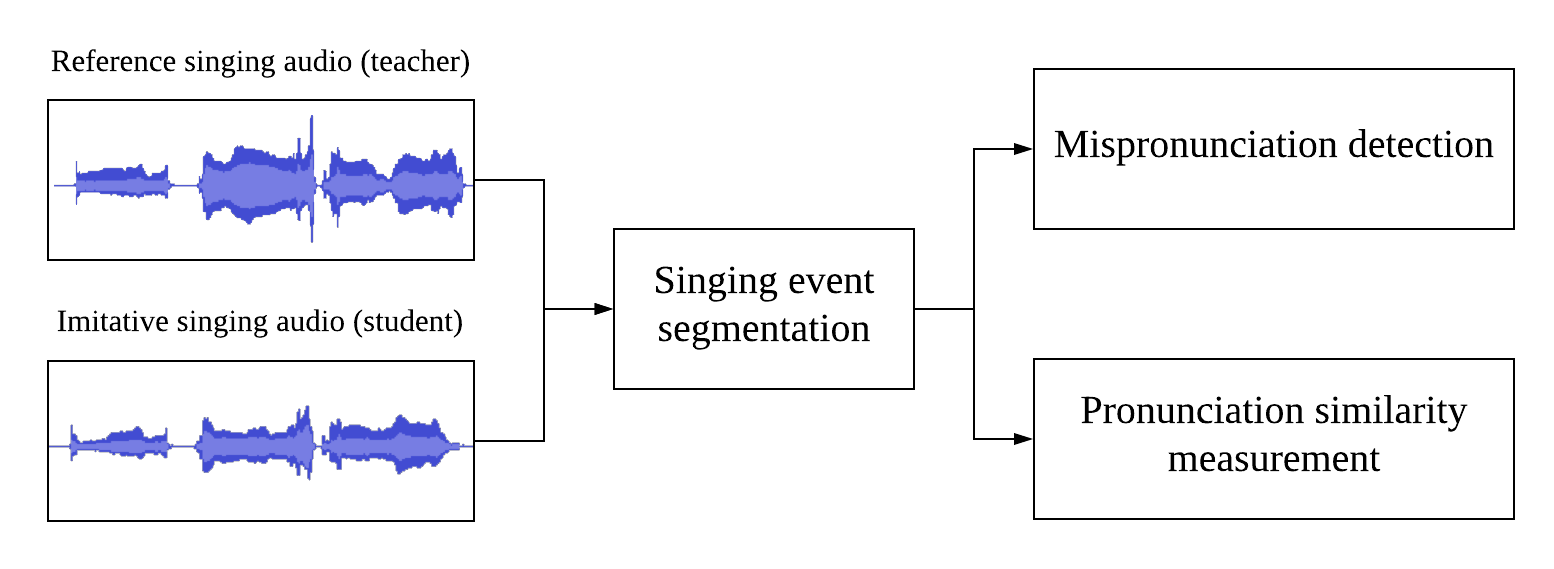
\includegraphics[scale=0.2]{figs/blockDiags_rong/ch1_motivation_audio.png}
\caption[Example of automatic singing voice assessment from the reference and imitative singing audio recordings]{Example of automatic singing voice assessment from the reference and imitative singing audio recordings, estimating singing event segments, detecting the mispronunciation and measuring the pronunciation similarity. The methods in this dissertation follows the similar diagram, with the audio recordings as the major information source.}\label{fig:intro:chapread}
\end{figure}

This dissertation investigates data-driven signal processing and machine learning approaches for automatic assessment of singing voice audio recordings. An audio recording is thus the primary source of information on which the computation models are built. \figref{fig:intro:chapread} shows an example of such diagram, presenting three assessment tasks - singing event segmentation, mispronunciation detection and pronunciation similarity measurement all adopt the audio recordings as the major information source. Other musical data sources such as musical scores, lyrics and editorial metadata are secondary, however, used in some tasks. The approaches adopted in this dissertation are mainly audio signal processing and machine learning (deep learning and probabilistic graphical models), investigating supervised learning methods to develop automatic singing voice assessment models.

This dissertation works toward to bring knowledge related to jingju music teaching and jingju music language to the methods. We aim to build knowledge-informed machine learning methods so that the extracted representations of the musical events and computational models are culturally relevant. High-level knowledge is taken as the determinants in the task and computational model designing.

The data-driven methods adopted in this dissertation require good quality and real-world data collections. We carefully collected, annotated and compiled the research datasets in align with the goal of building assessment models. The algorithms are developed to perform on the real world music teaching scenarios -- on the singing audio recordings of the actual classroom teaching.

The investigation in this dissertation is focused on developing novel automatic singing voice assessment methods and technologies, which are based on well-studied musicological knowledge of jingju music culture. Although the data and methods presented can eventually be adopted by musicologists for large-scale corpus analysis, the work does not aim to make any musicological contributions.

The musicological and music teaching knowledge adopted in this work is borrowed partly from the consultation with jingju performing teachers, students and jingju musicologists. The assessment models developed in this dissertation are by no means a replacement of expert music teachers, but only serve within the support of music teachers, musicologists, and as a guidance to jingju singing learners. In addition to developing novel approaches for automatic singing voice assessment, this dissertation aims to answer the following research questions:

\begin{enumerate}[leftmargin=*]
\item How do existing automatic music performance assessment methods developed within different musical context extend to jingju music? What limitations can we pinpoint from the current state of the art?
\item We assume the high-level musicological and music teaching knowledge is useful for defining research problems, tasks and helping design computational models. What kind of high-level knowledge are insightful? How and to what extent can such knowledge be used to achieve the goal?
\item It is hypothesized that music performance assessment is conducted on various musical or articulative event granularities and different musical dimensions. Which event granularities and which musical dimensions can bring new and unique challenges to this research topic, and in return, to generalise the existing state of the art methods?
\item What are machine learning methods or deep learning architectures which are able to learn the musical dimension-relevant representations on the variable-length musical events? What kind of side information is useful for the singing voice event segmentation and assessment? How can these side information be included in the machine learning framework?
\item It is assumed that the methods devised in this work are culture-specific. Generally, it is desirable to have a generalised method that can be transferred to other music cultures. How can the methods proposed in this work be adapted to a different music culture? 
\end{enumerate}

In general, this dissertation identifies the challenges and opportunities in automatic singing voice assessment of jingju music, formulates several assessment problems and tasks, tackles the issues with constructing datasets, and finally focus on the tasks of singing events segmentation, mispronunciation detection and pronunciation, overall quality similarity measurement. The scope of this dissertation within CompMusic is to support singing voice assessment methods and tools to be a part of the inclusive set of content-based analysis approaches.

One of the main advocacies of the CompMusic project is open and reproducible research -- openly sharing ideas, objectives, data, code and experimental results. All the data, code and experimental results presented in this dissertation will be openly accessible via open source platform (Github, Zenodo) under open and non-commercial licenses.

\section{Organization and thesis outline}

The dissertation has eight chapters. Each chapter is written on a main topic of the thesis and is aimed to be self-contained unit with introduction, main content and summary. After an introduction of the dissertation in \chapref{chap:intro}, \chapref{chap:bkgnd} presents an overview of the jingju music background and a state of the art review of the related research topics. \chapref{chap:probdef} is engaged in elucidating several new automatic singing voice assessment problems in jingju music. \chapref{chap:datasets} discusses the jingju music research corpora and mainly the a cappella singing voice datasets that will be used for several singing voice assessment tasks. \chapref{chap:segmentation}, \chapref{chap:similarity_pronunciation} and \chapref{chap:similarity_pronunciation} are the major chapters of this dissertation presenting the works of automatic singing syllable and phoneme segmentation, syllable-level mispronunciation detection and phoneme-level pronunciation similarity measurement. \chapref{chap:conclusions} presents applications, conclusions and future works. The links of external resources such as data, code are listed in \appref{app:resources}. 
% Jingju music-related terms and technical acronyms used in the dissertation are listed as a glossary in Appendix C. 

\chapref{chap:bkgnd} provides the necessary music and technical background for understanding the work presented in the thesis. We establish a consistent terminology for jingju music concepts. We describe pronunciation related concepts in jingju singing. We present an overview of the state of the art for the automatic singing voice pronunciation assessment problem tackled in the thesis. And finally we describe the technical concepts necessary to understand the algorithms and methods presented in this thesis.

\chapref{chap:probdef} presents the attempts to open up the research topic of automatic singing voice assessment. We first elucidate the important role of pronunciation played in jingju singing training. Then we introduce several relevant research problems, with a review of the state of the art for jingju music or other music traditions in the context of CompMusic project. We present the background of all the relevant research problems. We formulate the thesis problems of syllable and phoneme segmentation, mispronunciation detection for special pronunciation, and pronunciation similarity measures at phoneme level.

In \chapref{chap:datasets}, we compile and analyse the research corpus and test datasets for the research of this dissertation. We will discuss the corpus building criteria and evaluation methodologies. We describe the corpus and the test datasets, emphasizing the research problems and tasks relevant to this thesis. We describe a set of corpus design criteria and methodologies, then use them to evaluate the jingju a cappella singing voice corpus. We present both corpus-level and test dataset-level musically meaning data analysis and visualization. We mainly emphasize on presenting a scientific approach for corpus building and the evaluation of its coverage and completeness. Apart from the corpus description, the musically meaningful data analysis and visualization is another contribution of this chapter. Finally, the research corpus and test datasets presented in this chapter will be made available for further jingju \gls{MIR} research.

\chapref{chap:segmentation} aims to address the automatic syllable and phoneme segmentation task within the context of jingju music, presenting several methods and an evaluation of these methods. The problem is formulated in two ways -- duration-informed lyrics-to-audio alignment and duration-informed syllable or phoneme onset detection. Several approaches are proposed to address the problem. We present a detailed description of \gls{HSMM}-based segmentation method and the proposed onset detection-based method for syllable and phoneme segmentation. Finally, we present an evaluation of \gls{HSMM}-based alignment method and the proposed onset detection-based method and explore various deep learning architectures to improve the onset detection-based method.

\chapref{chap:mispronunciation} aims to address the automatic mispronunciation detection task within the context of jingju singing, presenting several methods and an evaluation of these methods. The problem is formulated as building discriminative machine learning models to classify binarily the singing syllables into mispronounced or correctly pronounced class. Several neural network architectures are experimented to address this problem. We present a description of the forced alignment-based baseline method and the discriminative model-based method for mispronunciation detection. We present an evaluation of the forced alignment-based method and the discriminative model-based method, and explore two deep learning architectures intending to improve the discriminative detection model. 

\chapref{chap:similarity_pronunciation} aims to address the pronunciation and overall quality similarities measurement task in the context of jingju singing training, presenting several methods and an evaluation of these methods. The problem is formulated as building machine learning models to perform phoneme embedding regarding pronunciation and overall quality aspects. Several neural network architectures are experimented to address this problem. We present a description of the classification model for phoneme embedding, and to explore the siamese network model for the same purpose. Finally, we present an evaluation of the classification model and the siamese model.

\chapref{chap:conclusions} presents some of the applications, conclusions, and the pointers for future work.

To our knowledge, this thesis is the first attempt at singing voice pronunciation assessment of jingju music. By tacking the problems presented in this thesis, we aim to develop useful tools and algorithms for automatic singing voice assessment of jingju music. In this process, we also hope to obtain a better understanding into the nature of pronunciation in jingju singing, and contribute to improving the state of the art.

%TODO: for each chapter, use one paragraph to describe the outline 

